\section{Model Free Reinforcement Learning}
\label{sec:mf_rl}

Model based methods are based on solving bellman equation \eqref{eqn:bellman_v}, \eqref{eqn:bellman_q} with given model $T$. 
On the other hand, Model Free Reinforcement Learning is suitable 
if environment model is not available but agent can experience environment by consequences of its actions. There are 3 main types. 

\begin{description}
	\item[Value Based Learning] Value functions are learned, 
	then policy arises naturally from value function as shown in \eqref{eqn:policy_stochastic_q} and \eqref{eqn:policy_deterministic_q}. 
	Since $\argmax$ operation is used, this type of learning is suitable for problems where action space is discrete. 
	
	\item[Policy Based Learning] Policy is learned directly, 
	return values are used instead of learning a value function. 
	Unlike value based methods, it is suitable for continious action spaces. 
	
	\item[Actor Critic Learning] Both policy (actor) and value (critic) functions are learned simulatenously. 
	It is also suitable for continious action spaces. 
	
\end{description}

\subsection{Q Learning}
Q Learning is a value based type of learning. 
It is based on optimizing $Q$ function using Bellman Equation \eqref{eqn:bellman_q}~\cite{watkins_technical_1992}. 
Assume that $Q$ function is parametrized by $\theta$. 
Target $Q$ value is estimated by bootstrapping estimate itself, 
\begin{equation}
\label{eqn:q_target}
Y_t^Q = r_t + \gamma \max_{a'} Q(s_{t+1},a';\theta).
\end{equation}
At time $t$,  with state, action, reward, next state tuples ($s_t,a_t,r_t,s_{t+1}$), 
$Q$ values are updated by minimizing difference between target value and estimated value, which is loss 
\begin{equation}
\label{eqn:q_loss}
\mathcal{L}_t(\theta) = \big( Y_t - Q(s_t,a_t;\theta) \big) ^ 2, 
\end{equation}
with respect to $\theta$ using numerical optimization methods. 

\subsubsection{Deep Q Learning}
Deep Q Learning overcomes instability of Q Learning, using Deep Q Network (DQN). 
When a nonlinear approximator is used, learning is unstable. 
Deep Q Learning introduces Target Network and Experience Replay \cite{mnih_human-level_2015, mnih_playing_2013}. 

\textbf{Target Network} is parametrized by $\theta^-$. 
It is used to evaluate target value and not updated by loss minimization. 
It is updated at each fixed number of update step $C$ by Q network parameter $\theta$. 
Target value is obtained by using $\theta^-$, 
\begin{equation}
\label{eqn:dqn_ntarget}
Y_t^{DQN} = r_t + \gamma \max_{a'} Q(s_{t+1},a';\theta^-).
\end{equation}

\textbf{Experience Replay} stores experience tuples in a replay memory $\mathcal{D}$ as queue with fixed buffer size $N_{replay}$. 
At each iteration $i$, $\theta$ is updated by experiences uniformly subsampled from experience replay by minimizing loss
\begin{equation}
\label{eqn:dqn_loss}
\mathcal{L}_i(\theta_i) = \mathbb{E}_{s,a,r,s'\sim U(\mathcal{D})}\Big[\big( Y^{DQN} - Q(s,a;\theta_i) \big) ^ 2 \Big].
\end{equation}
It allows agent to learn from experiences multiple times at different stages of learning. More importantly, sampled experiences are close to be independent and identically distributed if buffer size is high enough. 
This makes learning process more stable. 

As stated in \chapref{sec:chal}, exploration is an important step for reinforcement learning algorithms. 
\textbf{Epsilon Greedy Exploration} is used to let agent explore environment. 
In discrete action space (finite action space $\mathcal{A}$), this is 
simplest exploration strategy.
During learning, a random action is selected by probability $\epsilon$ or greedy action (maximizing Q value) by $1-\epsilon$. Mathematically,  
\begin{equation}
\label{eqn:egreedy_policy}
\pi(a|s) = 
\begin{cases}
1-\epsilon,   & \text{if } a = \argmax_{a} Q(s, a)\\
\frac{\epsilon}{|\mathcal{A}|-1},     & \text{otherwise}
\end{cases}.
\end{equation}

Algorithm is summarized in Algorithm \ref{alg:dqn}. 
\begin{algorithm}
	\SetAlgoLined
	\DontPrintSemicolon % Some LaTeX compilers require you to use \dontprintsemicolon instead
	Initialize: Replay memory $\mathcal{D}$ with capacity $N_{replay}$ \\
	Action value function parameters $\theta$ \\
	Target action value function parameters $\theta^- \leftarrow \theta$ \\
	Epsilon parameter for exploration $\epsilon$, Update delay parameter $d$ \\
	\For{$\text{episode} = 1, M $}{
		Recieve initial state $s_1$; \\
		\For{$t = 1, T$}{
			Select random action $a_t$ with probability $\epsilon$, otherwise greedy action $a_t = \arg\max_{a} Q(s_t, a; \theta)$; \\
			Execute action $a_t$ and recieve reward $r_t$ and next state $s_{t+1}$; \\
			Store experience tuple $e_t = (s_t, a_t, r_t, s_{t+1})$ to $\mathcal{D}$ ; \\
			Sample random batch with $N$ transitions from $\mathcal{D}$ as $\mathcal{D}_{r}$; \\
			$\forall e_j \in \mathcal{D}_{r}$, Set \\$Y_j = \begin{cases}
			r_j & \text{if } s_{j+1} \text{ terminal} \\
			r_j + \gamma \max_{a'} Q(s_{j+1},a';\theta^-) & \text{else}
			\end{cases}$; \\
			Update $\theta$ by minimizing $ \frac{1}{N}\sum_{e_j \in \mathcal{D}_{r}} \big( Y_j - Q(s_j,a_j;\theta) \big) ^ 2$ with a single optimization step; \\
			\lIf{$t \mod d$}{
				Update target network: $\theta^- \leftarrow \theta$;
			}
		}
	}
	\caption{Deep Q Learning with Experience Replay}
	\label{alg:dqn}
\end{algorithm}

\subsubsection{Double Deep Q Learning}
In DQN, max operator is used to select and evaluate action on the same network as in \eqref{eqn:dqn_ntarget}. 
This yields overestimated value estimations in noisy environments. 
Therefore, action selection and value estimation is decoupled in target evaluation 
to overcome $Q$ function overestimation~\cite{van_hasselt_deep_2015} using Double Deep Q Network (DDQN). The target value is
\begin{equation}
\label{eqn:ddqn_ntarget}
Y_t^{DDQN} = r_t + \gamma Q(s_{t+1}, \arg\max_{a'} Q(s_{t+1}, a'; \theta_i );\theta^-).
\end{equation}
Learning process is same with DQN except target value. 

\subsection{Actor Critic Learning}

Value based methods are not suitable for continious action spaces. 
Therefore, policy is explicitly defined instead of maximizing $Q$ function. 
For such problems, actor-critic type learning methods which uses both value and policy models seperately. 
Policy functions can be either stochastic or deterministic as stated in \chapref{sec:policy_control}.  

In actor-critic learning, there exist two components. 
First is actor, which is policy function which is either stochastic or deterministic and parametrized by $\theta^{\pi}$ or $\theta^{\mu}$. 
For policy learning, an estimate of value function is used instead of true value function since it is unknown. 
The estimate of value is calculated by critic parametrized by $\theta^Q$, which is second component~\cite{silver_deterministic_2014}. 
Critic learning is done by error minimization by several methods such as monte carlo sampling or temporal difference bootstrapping.

The ultimate goal is to maximize value function $V$. Therefore, policy is selection of action which maximizes $Q$ value as in \eqref{eqn:policy_deterministic_q}. 
Therefore, value function is the criteria to be maximized by solving parameters $\theta^\mu$ given $\theta^Q$. At time $t$, loss function for policy is negative value, in other words,  
\begin{equation}
\label{eqn:ac_value_maximization}
\mathcal{L}_t(\theta^\pi) = - Q(s_t, \widetilde{a}_t;\theta^Q), \quad \widetilde{a}_t \sim \pi(\cdot|s_t;\theta^\pi).
\end{equation}

In order to learn policy $\pi$, $Q$ function should also be learned simulatenously. 
For $Q$ function approximation, target value is parametrized by $\theta^Q$ and $\theta^\mu$,
\begin{equation}
\label{eqn:ac_target}
Y_t^{AC} = r_t + \gamma Q(s_{t+1}, \widetilde{a}_{t+1});\theta^Q), \quad \widetilde{a}_{t+1} \sim \pi(\cdot|s_{t+1};\theta^{\pi}).
\end{equation}
And this target is used to learn $Q$ function by minimizing least squares loss,
\begin{equation}
\label{eqn:ac_loss}
\mathcal{L}_t(\theta^Q) = \big( Y_t^{AC} - Q(s_t,a_t;\theta^Q) \big) ^ 2.
\end{equation}

Note that both actor and critic should be learned at the same time. Therefore, parameters are updated simulatenously during learning iterations. 

\subsubsection{Deep Deterministic Policy Gradient}
Deep Deterministic Policy Gradient (DDPG) is continuous compliment of DQN using deterministic policy~\cite{lillicrap_continuous_2019}. 
It also uses experience replay and target networks. 
Similar to Deep Q Learning, there are target networks parametrized by $\theta^{\mu^-}$ and $\theta^{Q^-}$ 
along with main networks parametrized by $\theta^{\mu}$ and $\theta^{Q}$. 

While target networks are updated in fixed number of steps in DQN, 
DDPG updates target network parameters at each step with polyak averaging, 
\begin{equation}
\label{eqn:target_update}
\theta^- \leftarrow \tau \theta + (1-\tau) \theta^- .
\end{equation}
The $\tau$ is an hyperparameter indicating how slow the target network is updated and usually close to zero. 

Policy network parameters are learned by maximizing resulting expected value, or minimizing its negative,
\begin{equation}
\label{eqn:ddpg_policy_loss}
\mathcal{L}_i(\theta^\mu_i) = \mathbb{E}_{s \sim U(\mathcal{D})} \Big[ -Q(s, \mu(s_t;\theta^\mu_i);\theta^Q) \Big].
\end{equation} 
Note that value network parameters are also assumed to be learned. 

Target networks are used to predict target value. Target is defined as 
\begin{equation}
\label{eqn:ddpg_target}
Y_t^{DDPG} = r_t + \gamma Q(s_{t+1}, \mu(s_{t+1};\theta^{\mu^-});\theta^{Q^-}).
\end{equation}
In each iteration, this target is used to learn $Q$ function by minimizing least squares loss, 
\begin{equation}
\label{eqn:ddpg_loss}
\mathcal{L}_i(\theta^Q_i) = \mathbb{E}_{s,a,r,s'\sim U(\mathcal{D})}\Big[\big( Y^{DDPG} - Q(s,a;\theta^Q_i) \big) ^ 2 \Big].
\end{equation}

In DDPG, value and policy network parameters are learned simultaneously. 
During learning, exploration noise is added to each selection. 
In original paper~\cite{lillicrap_continuous_2019}, authors proposed to use Ornstein Uhlenbeck Noise~\cite{uhlenbeck_theory_1930} which has temporal correlation for efficiency. 
However, simple gaussian noise or another noise is also possible. 

Algorithm is summarized in Algorithm \ref{alg:ddpg}. 
\begin{algorithm}
	\SetAlgoLined
	\DontPrintSemicolon % Some LaTeX compilers require you to use \dontprintsemicolon instead
	Initialize: Replay memory $\mathcal{D}$ with capacity $N_{replay}$ \\
	Policy and action value function parameters $\theta^{\mu}$, $\theta^Q$ \\
	Target policy and action value function parameters $\theta^{\mu^-} \leftarrow \theta^{\mu}$, $\theta^{Q^-} \leftarrow \theta^{Q}$ \\
	Random process $\mathcal{X}$ as exploration noise\\
	\For{$\text{episode} = 1, M $}{
		Recieve initial state $s_1$; \\
		\For{$t = 1, T$}{
			Select action $a_t = \mu(s_t; \theta^{\mu}) + \epsilon$ where $\epsilon \sim \mathcal{X}$; \\
			Execute action $a_t$ and recieve reward $r_t$ and next state $s_{t+1}$; \\
			Store experience tuple $e_t = (s_t, a_t, r_t, s_{t+1})$ to $\mathcal{D}$ ; \\
			Sample random batch with $N$ transitions from $\mathcal{D}$ as $\mathcal{D}_{r}$; \\
			$\forall e_j \in \mathcal{D}_{r}$, Set \\$Y_j = \begin{cases}
			r_j & \text{if } s_{j+1} \text{ terminal } \\
			r_j + \gamma Q(s_{j+1},\mu(s_{j+1}; \theta^{\mu^-}); \theta^{Q^-}) & \text{else}
			\end{cases}$; \\
			Update $\theta^Q$ by minimizing $ \frac{1}{N}\sum_{e_j \in \mathcal{D}_{r}} \big( Y_j - Q(s_j,a_j;\theta^Q) \big) ^ 2$ with a single optimization step; \\
			Update $\theta^{\mu}$ by maximizing $ \frac{1}{N}\sum_{e_j \in \mathcal{D}_{r}} Q(s_j,a_j;\theta^Q)$ with a single optimization step; \\
			Update target networks \\
			$\theta^{\mu^-} \leftarrow \tau \theta^{\mu} + (1-\tau) \theta^{\mu^-}$ \\
			$\theta^{Q^-} \leftarrow \tau \theta^{Q} + (1-\tau) \theta^{Q^-}$;
		}
	}
	\caption{Deep Deterministic Policy Gradient}
	\label{alg:ddpg}
\end{algorithm}

\textbf{Ornstein-Uhlenbeck Process} is continious analogue of discrete first order autoregressive (AR(1)) process~\cite{uhlenbeck_theory_1930}. 
The process $x$ is defined by a stochastic differential equation,
\begin{equation}
\label{eqn:ou_process}
\frac{dx}{dt} = -\theta x + \sigma \eta(t),
\end{equation}
where $\eta(t)$ is white noise. 
Its standard deviation in time is equal to $\frac{\sigma}{\sqrt{2\theta}}$. 
This process is commonly used as exploration noise in physical environments since it has momentum in time. 
A sample with different parameters is visualized in \figref{fig:ou_vs_gaussian}.

\begin{figure}
	\centering
	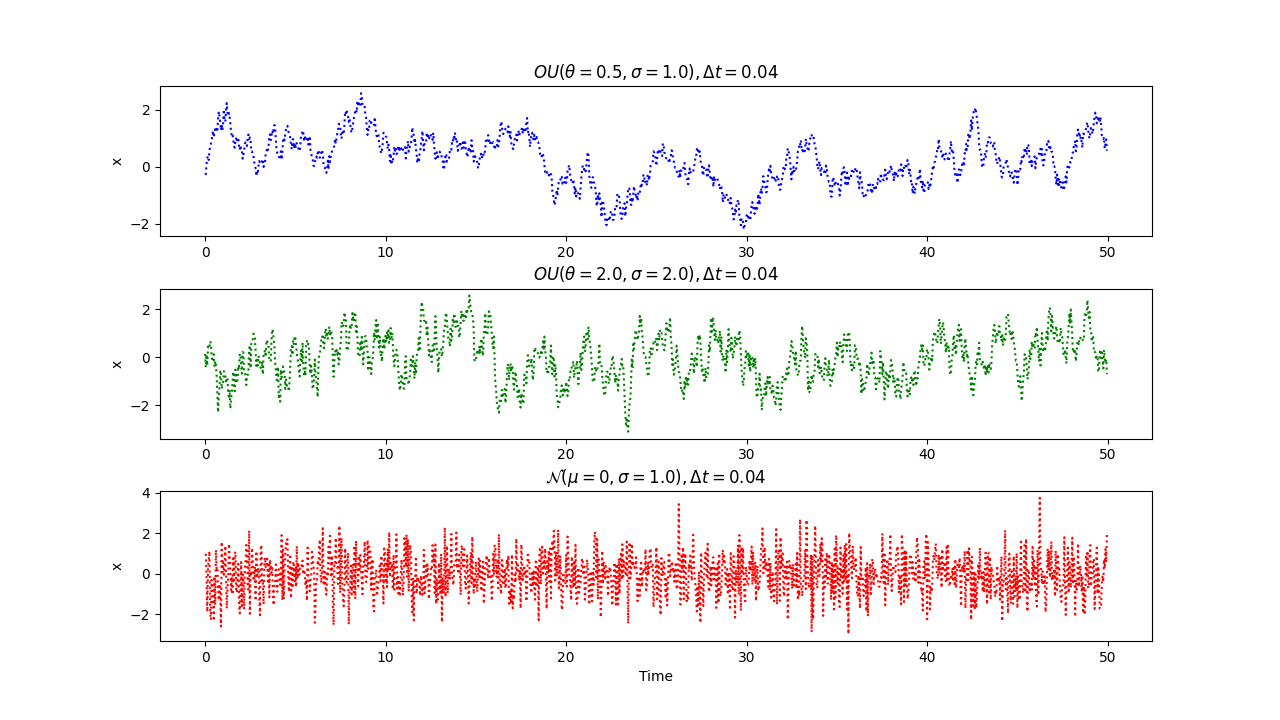
\includegraphics[width=0.98\textwidth]{figures/others/random_processes.png}
	\caption{Ornstein-Uhlenbeck Process and Gaussian Process comparison}
	\label{fig:ou_vs_gaussian}
\end{figure}

\subsubsection{Twin Delayed Deep Deterministic Policy Gradient}
Twin Delayed Deep Deterministic Policy Gradient (TD3)~\cite{fujimoto_addressing_2018} is improved version of DDPG with higher stability and efficiency. 
There are three main tricks upon DDPG. 

\textbf{Target Policy Smoothing} to regularize learning process by smoothing effects of actions on value. For target value assesing, actions are obtained from target policy network in DDPG, while a clipped zero centered gaussian noise is added to actions in TD3 as follows,
\begin{equation}
\label{eqn:td3_target_action}
\widetilde{a}' = \mu(s';\theta^{\mu^-}) + \text{clip}(\epsilon, -c, c), \quad \epsilon \sim \mathcal{N}(0, \sigma).
\end{equation}

\textbf{Clipped Double Q Learning} to escape from $Q$ value overestimation. 
There are two different $Q$ networks with their targets. 
During learning, both of them are learned from single target value. 
This value is assessed by using whichever of two networks give smaller of it. In other words, 
\begin{equation}
\label{eqn:td3_target}
Y_t^{TD3} = r_t + \gamma \min_{k\in\{1,2\}} Q(s_{t+1}, ;\widetilde{a}_{j+1};\theta^{Q_k^-}).
\end{equation}
However, policy is learned by maximizing output of first value network, or minimizing its negative,
\begin{equation}
\label{eqn:td3_policy_loss}
\mathcal{L}_i(\theta^\mu_i) = \mathbb{E}_{s \sim U(\mathcal{D})} \Big[ -Q(s, \mu(s;\theta^\mu_i);\theta^{Q_1}) \Big].
\end{equation} 

\textbf{Delayed Policy Updates} for stable training. 
During learning, policy network and target networks are updated less frequently (at each fixed number of step) than value network. 
Since policy network parameters are learned by maximizing value network, it should be learned slower. 

Algorithm is summarized in Algorithm \ref{alg:td3}. 
\begin{algorithm}
	\SetAlgoLined
	\DontPrintSemicolon % Some LaTeX compilers require you to use \dontprintsemicolon instead
	Initialize: Replay memory $\mathcal{D}$ with capacity $N_{replay}$ \\
	Policy and action value function parameters $\theta^{\mu}$, $\theta^Q_1$, $\theta^Q_2$  \\
	Target policy and action value function parameters $\theta^{\mu^-} \leftarrow \theta^{\mu}$, $\theta^{Q^-}_1 \leftarrow \theta^{Q}_1$, $\theta^{Q^-}_2 \leftarrow \theta^{Q}_2$ \\
	Random process $\mathcal{X}$ as exploration noise \\
	Target policy smoothing parameters $\sigma$, $c$, Update delay parameter $d$ \\
	\For{$\text{episode} = 1, M $}{
		Recieve initial state $s_1$; \\
		\For{$t = 1, T$}{
			Select action $a_t = \mu(s_t; \theta^{\mu}) + \epsilon$ where $\epsilon \sim \mathcal{X}$
			Execute action $a_t$ and recieve reward $r_t$ and next state $s_{t+1}$; \\
			Store experience tuple $e_t = (s_t, a_t, r_t, s_{t+1})$ to $\mathcal{D}$ ; \\
			Sample random batch with $N$ transitions from $\mathcal{D}$ as $\mathcal{D}_{r}$; \\
			Sample target actions for value target
			$\widetilde{a}_{j+1} = \mu(s_{j+1};\theta^{\mu^-}) + \text{clip}(\epsilon, -c, c), \quad \epsilon \sim \mathcal{N}(0, \sigma) \quad \forall e_j \in \mathcal{D}_{r}$; \\
			$\forall e_j \in \mathcal{D}_{r}$, $\forall k \in \{1,2\}$, Set \\
			$Y_{jk} = \begin{cases}
			r_j & \text{if } s_{j+1} \text{ terminal } \\
			r_j + \gamma Q(s_{j+1},\widetilde{a}_{j+1}); \theta^{Q^-}_k) & \text{else} 
			\end{cases}$; \\
			Set $Y_j = \min(Y_{j1}, Y_{j2})$; \\
			Update $\theta^Q_1$ $\theta^Q_2$ by seperately minimizing $ \frac{1}{N}\sum_{e_j \in \mathcal{D}_{r}} \big( Y_j - Q(s_j,a_j;\theta^Q_k) \big) ^ 2 \quad \forall k \in \{1,2\}$ with a single optimization step; \\
			\uIf{$t \mod d$}{
				Update $\theta^{\mu}$ by maximizing $ \frac{1}{N}\sum_{e_j \in \mathcal{D}_{r}} Q(s_j,a_j;\theta^Q_1)$ with a single optimization step; \\
				Update target networks \\
				$\theta^{\mu^-} \leftarrow \tau \theta^{\mu} + (1-\tau) \theta^{\mu^-}$ \\
				$\theta^{Q^-}_k \leftarrow \tau \theta^{Q}_k + (1-\tau) \theta^{Q^-}_k \quad \forall k \in \{1,2\}$ ;
			}
		}
	}
	\caption{Twin Delayed Deep Deterministic Policy Gradient}
	\label{alg:td3}
\end{algorithm}

%%%%%%%%%%%%%%%%%%%%%%
%%% NOT READY YET! %%%
%%%%%%%%%%%%%%%%%%%%%%

\subsubsection{Soft Actor Critic}
Soft Actor Critic (SAC)~\cite{haarnoja_soft_2018} is as stochastic actor critic method and other characteristics are similar to TD3 and DDPG. Its main advantage is that it learns to maximize exploration with entropy regularization. 

SAC is an entropy regularized RL method. Such methods gives bonus reward to agent propotional to policy entropy. Given state $s$, entropy of a policy is defined as,
\begin{equation}
\label{eqn:policy_entropy}
H(\pi(\cdot|s)) = \mathbb{E}_{\widetilde{a}\sim\pi(\cdot|s)}[-\log(\pi(\widetilde{a}|s))]
\end{equation}

Given entropy coefficient $\alpha$, definition of state-action value function is redefined as,
\begin{equation}
\label{eqn:q_dfn_entreg}
Q^{\pi}(s,a) = \mathbb{E}_{\substack{s'\sim T(\cdot|s,a)\\\widetilde{a}'\sim \pi(\cdot|s')} } \Big[r + \gamma \Big(Q^{\pi}(s',\widetilde{a}') -\log(\pi(\widetilde{a}'|s') \Big) \Big]. %\quad \forall t = 0,1, ...
\end{equation}

This modification changes $Q$ value target definition of TD3 as,
\begin{equation}
\label{eqn:q_target_sac}
Y_t^{SAC} = r_t + \gamma \Big(\min_{k\in\{1,2\}} Q(s_{t+1}, ;\widetilde{a}_{t+1};\theta^{Q_k^-}) -\alpha\log(\pi(\widetilde{a}_{t+1}|s_{t+1})) \Big), \quad \widetilde{a}_{t+1} \sim \pi(\cdot|s_{t+1}).
\end{equation}
Unlike TD3, policy updated according to minimum value of $Q$, while in TD3, policy is updated according to first $Q$ network as in \eqref{eqn:td3_policy_loss}. Mathematically, 
\begin{equation}
\label{eqn:sac_policy_loss}
\mathcal{L}_i(\theta^\pi_i) = - \mathbb{E}_{\substack{s \sim U(\mathcal{D})\\\widetilde{a} \sim \pi(\cdot|s)}} \Big[ \min_{k\in\{1,2\}} Q(s, \widetilde{a};\theta^{Q_k^-}) - \alpha\log(\pi(\widetilde{a}|s;\theta^\pi_i)) \Big].
\end{equation}

Since policy function is stochastic in SAC, it must be parametrized probability disribution. Most common one is 
Squashed Gaussian policy to squash actions in $(-1,1)$ range by $\tanh$ function, which has parametrized mean and standart deviation, i.e $\theta^{\pi}=(\theta^{\mu}, \theta^{\sigma})$. Actions are sampled as,
\begin{equation}
\label{eqn:squashed_gp_sampling}
a(s) = \tanh(\mu(s; \theta^{\mu}) + \eta \odot \sigma(s; \theta^{\sigma})), \quad \eta \sim \mathcal{N}(0, I). 
\end{equation}

Lastly, SAC method does not include policy delay, target policy smoothing and target policy network. 
Algorithm is summarized in Algorithm \ref{alg:sac}.
\begin{algorithm}
	\SetAlgoLined
	\DontPrintSemicolon % Some LaTeX compilers require you to use \dontprintsemicolon instead
	Initialize: Replay memory $\mathcal{D}$ with capacity $N_{replay}$ \\
	Policy and action value function parameters $\theta^{\pi}$, $\theta^Q_1$, $\theta^Q_2$  \\
	Target action value function parameters $\theta^{Q^-}_1 \leftarrow \theta^{Q}_1$, $\theta^{Q^-}_2 \leftarrow \theta^{Q}_2$ \\
	Entropy temperature $\alpha$ \\
	\For{$\text{episode} = 1, M $}{
		Recieve initial state $s_1$; \\
		\For{$t = 1, T$}{
			Select action $a_t \sim \pi(\cdot|s_t; \theta^\pi)$
			Execute action $a_t$ and recieve reward $r_t$ and next state $s_{t+1}$; \\
			Store experience tuple $e_t = (s_t, a_t, r_t, s_{t+1})$ to $\mathcal{D}$ ; \\
			Sample random batch with $N$ transitions from $\mathcal{D}$ as $\mathcal{D}_{r}$; \\
			Sample next actions for value target
			$\widetilde{a}_{j+1} \sim \pi(\cdot|s_{j+1};\theta^{\pi}) \quad \forall e_j \in \mathcal{D}_{r}$; \\
			$\forall e_j \in \mathcal{D}_{r}$, $\forall k \in \{1,2\}$, Set \\
			$Y_{jk} = \begin{cases}
			r_j & \text{if } s_{j+1} \text{ terminal} \\
			r_j + \gamma \Big(Q(s_{j+1},\widetilde{a}_{j+1}; \theta^{Q^-}_k) - \alpha\log(\widetilde{a}_{j+1} | s_{j+1}; \theta^\pi)\Big) &  \text{else}
			\end{cases}$; \\
			Set $Y_j = \min(Y_{j1}, Y_{j2})$; \\	
			Update $\theta^Q_1$ $\theta^Q_2$ by seperately minimizing $ \frac{1}{N}\sum_{e_j \in \mathcal{D}_{r}} \big( Y_j - Q(s_j,a_j;\theta^Q_k) \big) ^ 2 \quad \forall k \in \{1,2\}$ with a single optimization step; \\
			Sample actions for policy update,
			$\widetilde{a}_j \sim \pi(\cdot|s_j;\theta^{\pi}) \quad \forall e_j \in \mathcal{D}_{r}$; \\		
			Update $\theta^\pi$ by maximizing $ \frac{1}{N}\sum_{e_j \in \mathcal{D}_{r}} [\min_{k\in\{1,2\}} Q(s_j,\widetilde{a}_j;\theta^{Q_k})-\alpha\log(\pi(\widetilde{a}_j|s_j;\theta^\pi))]$ with a single optimization step; \\
			Update target networks \\
			$\theta^{Q^-}_k \leftarrow \tau \theta^{Q}_k + (1-\tau) \theta^{Q^-}_k \quad \forall k \in \{1,2\}$ ;

		}
	}
	\caption{Soft Actor Critic}
	\label{alg:sac}
\end{algorithm}
  
